\documentclass[conference]{IEEEtran}
\usepackage[utf8]{inputenc}
\usepackage[T1]{fontenc}
\usepackage{booktabs,tabularx,graphicx,url}
\title{VÉRTICE: una casa editorial de subastas curadas}
\author{\IEEEauthorblockN{Equipo del proyecto ECOMMERCE\_FRANK}}
\newcommand{\GaleriaLatencia}{%
\begin{table}[!ht]
\caption{Latencia HTTP de la galería en milisegundos}
\centering\footnotesize
\begin{tabular}{rrrrrrr}
\toprule
VU & Media & p95 & p99 & Máximo & req/s & Errores\\\midrule
3 & 63,65 & 245,67 & 793,87 & 4360,50 & 25,91 & 0\\
6 & 68,28 & 302,11 & 655,40 & 3268,34 & 45,58 & 1\\
8 & 46,39 & 245,80 & 508,74 & 1056,74 & 82,77 & 0\\
\bottomrule
\end{tabular}
\end{table}}
\newcommand{\GaleriaCobertura}{%
\begin{table}[!ht]
\caption{JaCoCo de líneas por servicio}
\centering\footnotesize
\begin{tabular}{lrr}
\toprule
Servicio & Unidad & Con integración\\\midrule
Auth & 20,29\,\% & 82,99\,\%\\
Catálogo & 33,14\,\% & 85,71\,\%\\
Notificaciones & 68,85\,\% & 82,62\,\%\\
Subastas & 16,08\,\% & 89,28\,\%\\
\bottomrule
\end{tabular}
\end{table}}
\newcommand{\GaleriaFlujos}{El lote 1411 registró dos postores y activó la extensión de cierre. La adjudicación 48 mantuvo la orden al repetir el pago. Mailpit recibió ambos avisos. La compra 3356 agotó la última unidad y recibió el correo. La actividad mostró ambos pagos y conservó su referencia al repetirse. La compra de edición 3503 verificó cupo y reintento concurrente.}
\newcommand{\GaleriaNewman}{Newman midió 90 peticiones con 0 errores HTTP y 11 aserciones fallidas de 269. Máximo de 1622,00 ms.}
\newcommand{\GaleriaDiagnostico}{En la medición previa a 8 VU, cambiar la clave consumió 234,77 ms por hash en promedio. PostgreSQL ejecutó el plan aislado de la portada en 0,529 ms. Los tiempos del arranque en frío se registraron aparte. El umbral por ruta y la cobertura unitaria del 80 \% siguen pendientes.}
\newcommand{\GaleriaPicos}{\paragraph{Picos por perfil.} 3 VU registró 7 rutas por encima de 500 ms. 6 VU registró 11 rutas por encima de 500 ms. 8 VU registró 6 rutas por encima de 500 ms. Los resultados adjuntos enumeran los máximos y p95 por ruta.}
\newcommand{\GaleriaRutas}{%
\begin{table}[!ht]
\caption{Máximos superiores a 500 ms}
\centering\scriptsize
\setlength{\tabcolsep}{3pt}
\begin{tabular}{llrrr}
\toprule
Servicio & Ruta & 3 VU & 6 VU & 8 VU\\\midrule
Auth & \texttt{POST /cambiar-clave} & 1935,41 & 3268,34 & 1056,74\\
Auth & \texttt{POST /login} & -- & -- & 799,24\\
Auth & \texttt{POST /renovar} & -- & 3006,68 & 832,97\\
Auth & \texttt{POST /save} & 573,64 & 3074,39 & 573,52\\
Catálogo & \texttt{DELETE /carrito/vaciar} & -- & 1194,16 & --\\
Catálogo & \texttt{DELETE /producto/:id} & -- & 1300,80 & --\\
Catálogo & \texttt{GET /compras} & 1236,84 & 1601,49 & 661,80\\
Catálogo & \texttt{GET /producto} & 994,45 & -- & --\\
Catálogo & \texttt{GET /producto/:id} & 1361,24 & -- & --\\
Catálogo & \texttt{GET /producto/entrega} & -- & 874,09 & --\\
Catálogo & \texttt{POST /carrito/agregar} & 2284,46 & -- & --\\
Catálogo & \texttt{POST /compras/realizar} & -- & -- & 591,28\\
Catálogo & \texttt{POST /producto} & 4360,50 & 698,14 & --\\
Catálogo & \texttt{PUT /producto/:id} & -- & 573,67 & --\\
Subastas & \texttt{GET /:id} & -- & 543,90 & --\\
Subastas & \texttt{GET /api/subastas/inicio} & -- & 510,15 & --\\

\bottomrule
\end{tabular}
\end{table}
}

\begin{document}
\maketitle
\begin{abstract}
VÉRTICE ofrece subastas curadas con un canal de compra directa. Cuatro servicios gestionan cuentas, catálogo, pujas y notificaciones sobre PostgreSQL. Se verificaron inventario, adjudicación, correo en Mailpit y latencia de 52 rutas. Los escenarios de 3, 6 y 8 usuarios virtuales midieron errores funcionales y el umbral académico de 500 ms por ruta.
\end{abstract}
\begin{IEEEkeywords}
comercio electrónico, subastas, microservicios, concurrencia, PostgreSQL
\end{IEEEkeywords}
\section{Introducción}
El inventario de una tienda necesita preservar el precio de una compra y evitar que dos personas adquieran la misma unidad. Una subasta exige resolver además quién ofrece el monto más alto en un plazo limitado. VÉRTICE reúne ambos recorridos en una galería de diseño y colección con precios en COP. En la tienda, la confirmación registra una compra y descuenta inventario en la misma transacción. En las subastas, la orden de adjudicación habilita un pago simulado. Los lotes de vehículos y joyería son ejemplos ficticios.

\section{Arquitectura y tecnologías}
Auth valida contraseñas, controla intentos de login y emite JWT. Catálogo administra información, filtros, inventario, carrito y compras. Subastas administra lotes, pujas, adjudicaciones y el pago simulado. Notificaciones prepara y envía avisos y conserva reintentos y cola de errores. Los cuatro servicios se ejecutan con Java 17 y Spring Boot. Los adaptadores permiten que el dominio y los casos de uso prescindan de dependencias Spring, JPA o AMQP. ArchUnit comprueba esa separación.

\begin{center}
\begin{tabular}{c}
React $\rightarrow$ Auth, Catálogo, Subastas\\
Auth, Catálogo, Subastas $\rightarrow$ RabbitMQ\\
RabbitMQ $\rightarrow$ Notificaciones $\rightarrow$ Mailpit/Brevo\\
Los cuatro servicios $\rightarrow$ PostgreSQL
\end{tabular}\\
Fig. 1. Componentes de VÉRTICE.
\end{center}

PostgreSQL conserva cuenta, producto, carrito, compra, lote, puja, adjudicación y avisos. La tabla de pujas y la orden referencian al lote. Los identificadores de usuario se usan como referencias lógicas a Auth. Catálogo usa Frankfurter para mostrar un equivalente en USD y Nager.Date para excluir festivos al calcular la entrega. Las consultas externas fallidas generan una respuesta con datos parciales o un aviso en la ficha.


\clearpage
\section{Reglas y concurrencia}
El administrador publica y cancela lotes. Las personas autenticadas pueden pujar. Una oferta debe alcanzar el precio vigente más el incremento y no puede superar la oferta propia cuando ya lidera. En los últimos dos minutos, una oferta aceptada prolonga el plazo dos minutos. La consulta pública devuelve precios y alias. Las órdenes se revelan únicamente al ganador.

El repositorio bloquea la fila del lote y comprueba la versión al modificarla. En una prueba con dos hilos y el mismo monto se registró una sola puja. La máquina de estados admite programada, activa, cerrada, adjudicada y cancelada. El cierre sin postores permanece cerrado. Si hay ganador, el proceso crea su orden y conserva el precio final. Confirmar nuevamente el pago simulado devuelve el mismo resultado.

El aviso de puja superada, salida próxima, ganadora o cierre sin ganador nace en la misma transacción que el cambio. El proceso de publicación espera confirmación de RabbitMQ y reintenta con espera creciente. La entrega al menos una vez admite duplicados si el proceso cae tras la confirmación del broker. Notificaciones consume la cola compartida y envía el correo.

\section{Metodología}
La evaluación usó una instalación Windows con PostgreSQL, RabbitMQ y Mailpit en ejecución. JaCoCo comprobó líneas ejecutadas por pruebas unitarias y de integración. Newman cubrió validación de contrato, tiempos y el flujo de dos postores. La prueba de navegador aceleró solo el reloj de un lote sintético para observar la tarea programada. Axe analizó el listado de lotes en tres anchos. k6 ejecutó carga con 3 usuarios y rampas a 6 y 8, con 52 rutas. El máximo por ruta evalúa el umbral académico.


\clearpage
\section{Resultados}
\GaleriaLatencia
\GaleriaFlujos

\GaleriaNewman

\begin{figure}[!ht]
\centering
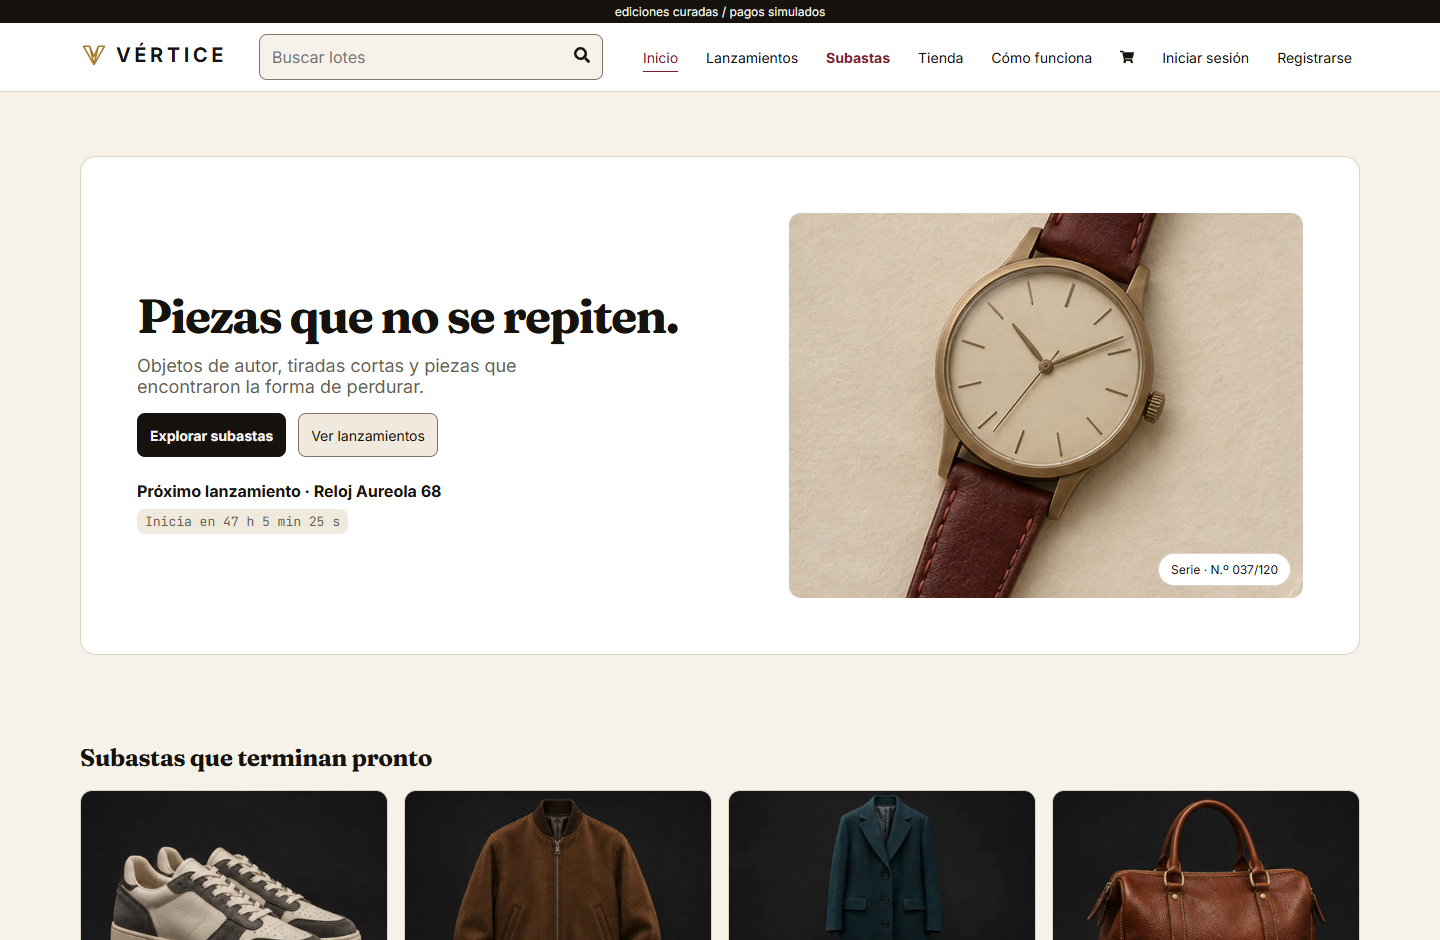
\includegraphics[width=.90\columnwidth]{../capturas/vertice-curado-portada.png}
\caption{Portada editorial dedicada a lotes de subasta.}
\end{figure}

\begin{figure}[!ht]
\centering
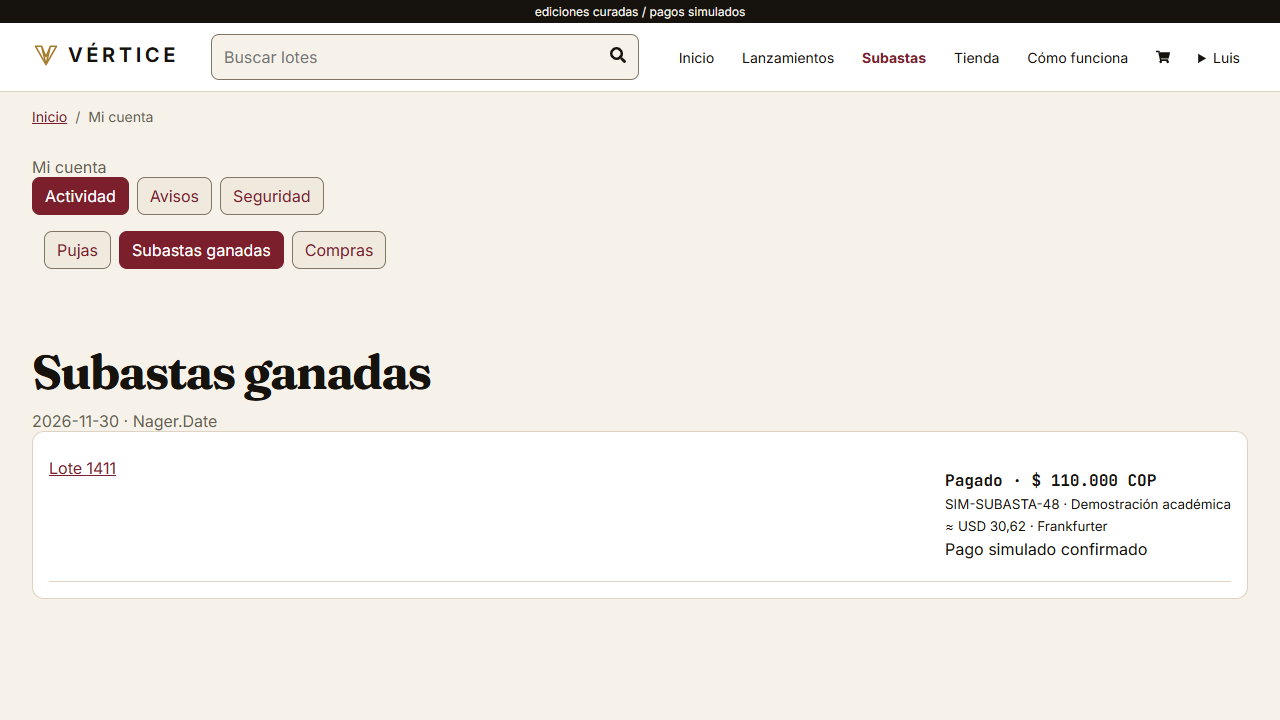
\includegraphics[width=.90\columnwidth]{../capturas/vertice-curado-puja-ganadas-pagada.png}
\caption{Adjudicación pagada desde la actividad de la cuenta.}
\end{figure}

\clearpage
\section{Despliegue y conclusiones}
La implementación local usa un script Windows. El Blueprint define cuatro servicios en Render con conexión TLS a Neon y AMQPS de CloudAMQP. Vercel sirve el frontend y Brevo suministra SMTP. El despliegue público requiere completar las cuentas del propietario. Render Free suspende procesos inactivos. Neon Free suspende su cómputo tras cinco minutos sin actividad \cite{render,neon}. El cierre programado actúa mientras el servicio está activo.

Los resultados verifican las transacciones, los avisos y la separación de responsabilidades. El umbral de 500 ms sigue pendiente en los perfiles medidos. La validación local tampoco mide la primera visita tras suspender los procesos en la nube. El siguiente paso consiste en separar las latencias de las consultas, la escritura, los hashes y la espera para localizar los picos y repetir perfiles comparables.

\subsection{Curaduría editorial y procedencia ilustrativa}
VÉRTICE ofrece 18 lotes distribuidos en siete categorías y tres ediciones limitadas. Las pruebas internas conservan sus datos y queda fuera de la galería cualquier ficha de ensayo. La actividad concentra pujas, adjudicaciones y compras. Catálogo y Subastas mantienen sus órdenes, con referencias estables y un único paso de pago simulado. Las referencias de entrega y conservación se muestran fuera del panel de puja.

Frankfurter ofrece COP/USD, Nager.Date estima días hábiles y Open-Meteo contextualiza temperatura y humedad. La actualización usa caché, timeout, reintento acotado y cortacircuito. Los pagos, entregas, procedencias y traspasos se simulan.

\GaleriaCobertura
\GaleriaDiagnostico

\begin{thebibliography}{00}
\bibitem{argon} A. Biryukov et al., RFC 9106, 2021. \url{https://www.rfc-editor.org/rfc/rfc9106}
\bibitem{render} Render, \emph{Deploy for Free}. \url{https://render.com/docs/free}
\bibitem{neon} Neon, \emph{Scale to Zero}. \url{https://neon.com/docs/introduction/scale-to-zero}
\bibitem{k6} Grafana Labs, \emph{k6 metrics reference}. \url{https://grafana.com/docs/k6/latest/using-k6/metrics/reference/}
\bibitem{meteo} Open-Meteo, \emph{Weather Forecast API}. \url{https://open-meteo.com/en/docs}
\end{thebibliography}
\end{document}
